Time-domain power thresholds detect attacks by magnitude, but
frequency-domain analysis can reveal periodic structure that
distinguishes adversarial duty cycling from legitimate workload
variation.  We compute Welch power-spectral-density (PSD) estimates
over each trial's power trace using 64-sample Hann-windowed segments
with 50\% overlap.  The effective sampling rate of the INA3221 polling
loop is $f_s \approx 3.8$\,Hz (Nyquist $\approx 1.9$\,Hz), so the
analysis resolves macro-level power oscillations below 2\,Hz---not the
configured 10\,kHz modulation frequency, which would require
instrumentation at $\ge$20\,kHz (see \S\ref{sec:discussion}).

\paragraph{Spectral energy separation.}
Table~\ref{tab:fft_features} reports four spectral features averaged
across five trials per condition.  The dominant finding is that attack
conditions concentrate dramatically more energy in the power spectrum
than baseline workloads.  At the highest clock cap (1575\,MHz), attack
spectral energy is 11.6$\times$ the baseline; at 630\,MHz it reaches
53.7$\times$.  Across all five oversubscription budget levels, a
Mann--Whitney $U$ test rejects the null hypothesis that baseline and
attack spectral energies are drawn from the same distribution
($U = 1$, $p = 0.016$).

In the contention-isolation experiment, the pattern holds regardless
of clock policy: fixed-clock attack energy is 26.2$\times$ baseline,
and default-clock attack energy is 37.8$\times$ baseline.  The higher
ratio under the default policy reflects the additional DVFS-induced
power variance as the governor responds to adversarial load cycling.

\paragraph{Spectral entropy.}
Spectral entropy measures how uniformly energy is distributed across
frequency bins.  For most oversubscription conditions, attack entropy
is comparable to or slightly lower than baseline (1.56--2.31 vs.\
1.76--4.06\,bits), indicating that the attacker's periodic structure
concentrates energy into fewer spectral modes rather than spreading it
broadband.  The 630\,MHz baseline is an exception (4.06\,bits)---its
low total energy yields a nearly flat, noise-dominated spectrum.

\paragraph{Implications for detection.}
These results confirm that even at the low temporal resolution of
sysfs-based power polling, frequency-domain features provide a
complementary detection signal.  A threshold on total spectral energy
alone achieves perfect separation in this dataset, and the spectral
centroid shift (lower under attack) suggests that adversarial power
oscillations are dominated by very-low-frequency components
($<$0.2\,Hz).  Figure~\ref{fig:fft_spectral} visualizes the PSD
curves, showing the order-of-magnitude separation between baseline and
attack conditions across representative clock caps and both clock
policies.

\begin{table}[t]
\centering
\footnotesize
\caption{Spectral features of GPU power traces under baseline and attack conditions. Total energy, entropy, and dominant frequency are computed from Welch PSD estimates (effective $f_s \approx 3.8$\,Hz, Nyquist $\approx 1.9$\,Hz).}
\label{tab:fft_features}
\begin{tabular}{llrrrr}
\toprule
Condition & State & Energy (W$^2$) & Entropy (bits) & Centroid (Hz) & Dom.\ Freq (Hz) \\
\midrule
\multicolumn{6}{l}{\textit{Power-budget oversubscription}} \\
  468MHz & Baseline & 2.3 & 1.95 & 0.135 & 0.070 \\
  468MHz & Attack & 3.3 & 2.31 & 0.158 & 0.067 \\
  630MHz & Baseline & 0.1 & 4.06 & 0.476 & 0.067 \\
  630MHz & Attack & 5.1 & 1.97 & 0.132 & 0.067 \\
  945MHz & Baseline & 1.5 & 2.07 & 0.154 & 0.067 \\
  945MHz & Attack & 8.8 & 2.05 & 0.126 & 0.065 \\
  1260MHz & Baseline & 4.0 & 2.09 & 0.142 & 0.066 \\
  1260MHz & Attack & 9.5 & 1.56 & 0.099 & 0.067 \\
  1575MHz & Baseline & 1.3 & 1.76 & 0.105 & 0.067 \\
  1575MHz & Attack & 15.4 & 1.94 & 0.101 & 0.066 \\
\midrule
\multicolumn{6}{l}{\textit{Contention isolation}} \\
  Fixed clock & Baseline & 2.2 & 2.59 & 0.174 & 0.061 \\
  Fixed clock & Attack & 58.1 & 2.72 & 0.195 & 0.062 \\
  Default clock & Baseline & 2.1 & 2.89 & 0.195 & 0.058 \\
  Default clock & Attack & 80.0 & 2.43 & 0.163 & 0.062 \\
\bottomrule
\end{tabular}
\end{table}


\begin{figure}[t]
  \centering
  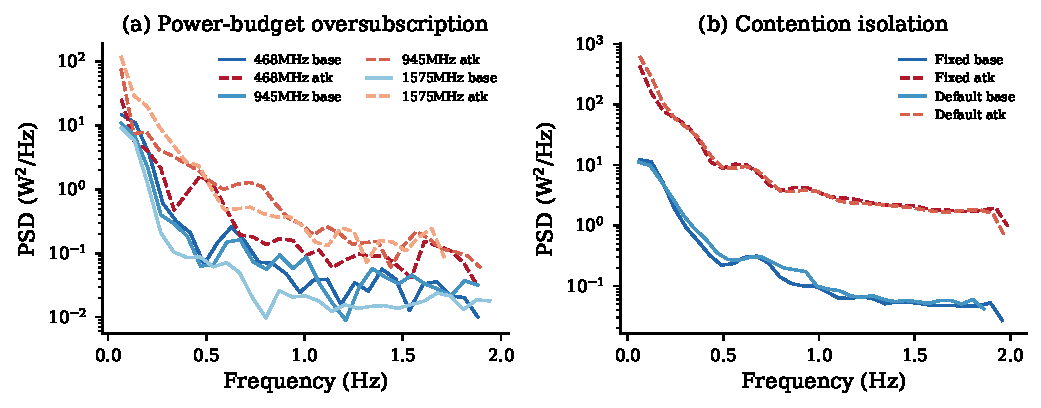
\includegraphics[width=\columnwidth]{figures/fig_fft_spectral.pdf}
  \caption{Power spectral density of GPU power traces.
    (a)~Oversubscription at three clock caps: attack conditions
    (dashed) show 1--2 orders of magnitude higher PSD than baseline
    (solid).
    (b)~Contention isolation under fixed and default clock policies:
    the DVFS-enabled default policy produces the highest spectral
    energy under attack.}
  \label{fig:fft_spectral}
\end{figure}
